\documentclass[12pt,a4paper]{article}
\usepackage[twoside]{fancyhdr}
\usepackage[utf8]{inputenc}
\usepackage{amsmath}
\usepackage{amsfonts}
\usepackage{amssymb}
\usepackage{polski}
\usepackage{indentfirst}
\usepackage{graphicx}
\usepackage{listings}
\usepackage{tikz}
\usepackage{blindtext}
\usepackage{multicol}
\usepackage{enumitem}   
\usepackage{listings}   %do kodów źródłowych
\usepackage{color}      %
\usepackage{tabularx}
\usepackage{float}
\usepackage{hyperref}

\definecolor{dkgreen}{rgb}{0,0.6,0}
\definecolor{gray}{rgb}{0.5,0.5,0.5}
\definecolor{mauve}{rgb}{0.58,0,0.82}

\lstset{frame=tb,       %ustawianie skłądni kodu
  language=C++,
  aboveskip=3mm,
  belowskip=3mm,
  showstringspaces=false,
  columns=flexible,
  basicstyle={\small\ttfamily},
  numbers=none,
  numberstyle=\tiny\color{gray},
  keywordstyle=\color{blue},
  commentstyle=\color{dkgreen},
  stringstyle=\color{mauve},
  breaklines=true,
  breakatwhitespace=true,
  tabsize=3
}


\begin{document}
%STRONA TYTUŁOWA
% \input{titlepage}

% \newpage
% \maketitle

\tableofcontents
\newpage


\setlength{\parindent}{0pt} %brak akapitów

\section{Przypadki użycia}

\subsection{Definicje aktorów}

% \begin{center}
    
\begin{table}[H]
\centerline{
\resizebox{1.4\textwidth}{!}{%
\begin{tabular}{|l|l|l|}
\hline
AKTOR & OPIS & PRZYPADKI UŻYCIA \\ \hline

Użytkownik niezarejestrowany & \begin{tabular}[c]{@{}l@{}} Osoba mogącą tylko założyć\\ konto klienta sklepu \end{tabular} & \begin{tabular}[c]{@{}l@{}}PU Create account \end{tabular} \\ \hline

Klient & \begin{tabular}[c]{@{}l@{}} Osoba przeglądająca\\ i pobierająca oprogramowanie\\ ze sklepu za darmo. \end{tabular} & \begin{tabular}[c]{@{}l@{}}
PU Search software powiązane przez \textless{}\textless{}include\textgreater{}\textgreater z:\\
$\cdot$PU Advanced-look at software\\
\\
PU Advanced-look at software powiązane przez \textless{}\textless{}extend\textgreater{}\textgreater z:\\ 
$\cdot$PU Report error,  \\ 
$\cdot$PU Download executable file,\\ 
$\cdot$PU Report violation, \\ 
oraz powiązane przez \textless{}\textless{}include\textgreater{}\textgreater z:\\
$\cdot$PU Look at review's and avarage of rating\\
\\
PU Look at review's and avarage of raiting powiązane przez \textless{}\textless{}extend\textgreater{}\textgreater z:\\ 
$\cdot$PU Add rating,  \\ 
$\cdot$PU Delete rating,\\ 
$\cdot$PU Create written review, \\ 
$\cdot$PU Edit written review, \\ 
$\cdot$PU Delete written review, \\
\\
PU Request administrator for change account to Software author \\ 

\end{tabular} \\ \hline

Autor oprogramowania & \begin{tabular}[c]{@{}l@{}} Osoba wgrywająca pliki\\ źródłowe do sklepu,\\ zarządzająca swoim oprogramowaniem \end{tabular} & \begin{tabular}[c]{@{}l@{}}
+ Przypadki użycia Klienta\\
...\\
PU Add new software,  \\ 
PU Read received bug reports, połączony przez \textless{}\textless{}extend\textgreater{}\textgreater z: \\ 
$\cdot$PU Close bug reports, \\ 
PU Delete software, \\ 
PU Update software, \\ 
\end{tabular} \\ \hline

Administrator & \begin{tabular}[c]{@{}l@{}} Osoba zarządzająca sklepem \\oraz użytkownikami.\\ Posiada najwyższy stopień uprawnień\end{tabular} & \begin{tabular}[c]{@{}l@{}}
+ Przypadki użycia Klienta\\
+ Przypadki użycia Autora oprogramowania\\
...\\
PU Read reports about violation,  \\ 
PU Close reports about violation,  \\ 
PU Block software from a shop,\\ 
PU Delete software from a shop, \\ 
PU Download software's source-code, \\ 
PU Analyse requests about changing accounts to Software author, \\ 
PU Delete Client's review, połączony przez \textless{}\textless{}extend\textgreater{}\textgreater z: \\
$\cdot$ PU Look at review's and avarage of raiting \\
\\
PU Delete User's account, \\ 
\end{tabular} \\ \hline

\end{tabular}%
}
}
\end{table}
% \end{center}



\subsection{Opis przypadków użycia Użytkownika niezajestrowanego}

\subsubsection{Create account}
\textbf{Cel: } Założenie konta w sklepie z oprogramowaniem \\
\textbf{Warunki wstępne: }Inicjalizacja przez uruchomienie aplikacji. \\
\textbf{Warunki końcowe: } Utworzenie konta w systemie lub wyświetlenie błędu o niepoprawnych danych \\
\textbf{Przebieg:}
\begin{enumerate}
    \item Należy przejść do formularza rejestracyjnego 
    \item Podanie danych do rejestracji:
    \begin{itemize}
        \item Imie
        \item Nazwisko
        \item Nickname
        \item E-mail
        \item Hasło (co najmniej 8 znaków)
        \item Data urodzenia
    \end{itemize}
    \item Jeśli podane dane są prawidłowe, użytkownik promowany jest automatycznie na \textbf{Klienta} oraz zostanie dodany do bazy danych. Jeśli nie są prawidłowe, to wyświetlany jest stosowny komunikat oświadczający, że wprowadzono niepoprawne dane.
\end{enumerate}



\subsection{Opis przypadków użycia Klienta}

% \begin{center}
%     \large{Pakiet przypadków użycia Klienta}
% \end{center}

\subsubsection{Add rating}
\textbf{Cel: } Ocenienie aplikacji w sklepie, w skali od 1-5  \\
\textbf{Warunki wstępne:} Inicjalizacja przez uruchomienie aplikacji, wyszukanie produktu, wybranie go oraz wejście w sekcje ocen za pomocą \textcolor{red}{PU Look at review's an avarage of raiting}.\\ Posiadanie uprawnień klienta lub wyższych.\\
\textbf{Warunki końcowe: } Wystawienie oceny aplikacji \\
\textbf{Przebieg:}
\begin{enumerate}
    \item W wybranym oprogramowaniu ze sklepu, wystawić ocenę za pomocą gwiazdek:
    \begin{itemize}
        \item 1 - $\star$
        \item 2 - $\star\star$
        \item 3 - $\star\star\star$
        \item 4 - $\star\star\star\star$
        \item 5 - $\star\star\star\star\star$
    \end{itemize}
    \item Dodanie oceny do bazy danych.
    \item Wyświetlenie komunikatu z podziękowaniami za wystawioną ocenę.
\end{enumerate}

\subsubsection{Delete rating}
\textbf{Cel: } Usunięcie oceny oprogramowania  \\
\textbf{Warunki wstępne: }Inicjalizacja przez uruchomienie aplikacji, wyszukanie oprogramowania, wejście w produkt, gdzie została już wystawiona ocena oraz w sekcje ocen za pomocą \textcolor{red}{PU Look at review's an avarage of raiting} \\ Posiadanie uprawnień klienta lub wyższych.\\
\textbf{Warunki końcowe: } Usunięcie oceny oprogramowania jeśli potwierdzono komunikat, jeśli nie, anulowanie funkcji\\
\textbf{Przebieg:}
\begin{enumerate}
    \item Przy wystawionej ocenie, kliknąć w znak \textit{X}
    \item Wyświetlenie komunikatu z zapytaniem o usunięciu oceny. (Czy chcesz usunąć ocenę?)
    \item Jeśli została wybrana opcja TAK, następuję usunięcie oceny ze sklepu oraz z bazy danych. Jeśli została wybrana opcja NIE, następuję tylko wyjście z komunikatu.
\end{enumerate}

\subsubsection{Create verbal review}
\textbf{Cel: } Utworzenie słownej recencji odnośnie oprogramowania \\
\textbf{Warunki wstępne:} Inicjalizacja przez uruchomienie aplikacji, wyszukanie oprogramowania, wejście w produkt, gdzie ma zostać wystawiona recenzja oraz w sekcje ocen za pomocą \textcolor{red}{PU Look at review's an avarage of raiting} \\ Posiadanie uprawnień klienta lub wyższych.\\
\textbf{Warunki końcowe:} Utworzenie recenzji jeśli potwierdzono komunikat, jeśli nie, anulowanie funkcji \\
\textbf{Przebieg:}
\begin{enumerate}
    \item Należy kliknąć znak \textit{+} w sekcji \textit{Opinie}
    \item Napisanie recenzji w specjalnie wydzielonym miejscu
    \item Zatwierdzenie recenzji poprzez wciśnięcie przycisku \textbf{Dodaj} oraz dodanie recenzji do bazy danych lub opuszczenie funkcji poprzez wciśnięcie przycisku \textbf{Anuluj}
\end{enumerate}

\subsubsection{Edit verbal review}
\textbf{Cel: } Edytowanie istniejącej już recenzji \\
\textbf{Warunki wstępne:} Inicjalizacja przez uruchomienie aplikacji, wyszukanie produktu, wejście w produkt, gdzie została już wystawiona ocena oraz w sekcje ocen za pomocą \textcolor{red}{PU Look at review's an avarage of raiting}\\ Posiadanie uprawnień klienta lub wyższych.\\ 
\textbf{Warunki końcowe:} Zmiana treści recenzji jeśli potwierdzono komunikat, jeśli nie, anulowanie funkcji \\
\textbf{Przebieg:}
\begin{enumerate}
    \item Należy kliknąć w przycisk \textbf{Edytuj} przy wystawionej recenzji
    \item Edytowanie treści recenzji
    \item Zatwierdzenie edytowania recenzji poprzez wciśnięcie przycisku \textbf{Zatwierdź} oraz zmiana recenzji w bazie danych lub opuszczenie funkcji poprzez wciśnięcie przycisku \textbf{Anuluj}
\end{enumerate}

\subsubsection{Delete verbal review}
\textbf{Cel: } Usunięcie istniejącej już recenzji \\
\textbf{Warunki wstępne:} Inicjalizacja przez uruchomienie aplikacji,  wyszukanie produktu, wejście w produkt, gdzie została już wystawiona ocena oraz w sekcje ocen za pomocą \textcolor{red}{PU Look at review's an avarage of raiting}\\ Posiadanie uprawnień klienta lub wyższych.\\
\textbf{Warunki końcowe:} Usunięcie recenzji jeśli potwierdzono komunikat, jeśli nie, anulowanie funkcji\\
\textbf{Przebieg:}
\begin{enumerate}
    \item Należy kliknąć w przycisk \textbf{Usuń} przy wystawionej recenzji
    \item Zatwierdzenie usunięcia recenzji poprzez wciśnięcie przycisku \textbf{Usuń} oraz usunięcie recenzji z bazy danych lub opuszczenie funkcji poprzez wciśnięcie przycisku \textbf{Anuluj}
\end{enumerate}

\subsubsection{Search software}
\textbf{Cel: } Poszukiwanie konkretnego oprogramowania \\
\textbf{Warunki wstępne:} Inicjalizacja przez uruchomienie aplikacji\\ Posiadanie uprawnień klienta lub wyższych.\\
\textbf{Warunki końcowe:} Znalezienie oprogramowania\\
\textbf{Przebieg:}
\begin{enumerate}
    \item Wyświetlenie listy dostępnych aplikacji oraz pola do wpisywania nazwy oprogramowania
    \item Należy wpisać nazwę poszukiwanego oprogramowania, w celu ograniczenia liczby wyświetlanych programów lub wybrać z listy konkretną pozycję z oprogramowaniem
    \item Po wybraniu konkretnej pozycji, następuję przejście do widoku danego oprogramowania za pomocą \textcolor{red}{PU Advanced-look at software}
\end{enumerate}

\subsubsection{Advanced-look at software}
\textbf{Cel: } Przeglądanie informacji o oprogramowaniu \\
\textbf{Warunki wstępne:} Inicjalizacja przez uruchomienie aplikacji, wybranie oprogramowania za pomocą \textcolor{red}{PU Search software}\\ Posiadanie uprawnień klienta lub wyższych.\\
\textbf{Warunki końcowe:} Znalezienie oprogramowania oraz wyświetlenie informacji z nim związanych lub wykonanie czynności związanych z recenzją/pobraniem/zgłoszeniem \\
\textbf{Przebieg:}
\begin{enumerate}
    \item Wyświetlenie informacji o oprogramowaniu:
    \begin{itemize}
        \item Nazwy
        \item Kategoria
        \item Grafiki przedstawiającej oprogramowanie
        \item Opisu
        \item Autora
        \item Recenzji za pomocą \textcolor{red}{PU Look at review's and avarage of raiting}
    \end{itemize}
    \item Możliwość przejścia do innych opcji:
    \begin{itemize}
        \item Zgłoszenia błędu w oprogramowaniu za pomocą: \textcolor{red}{PU Report error}
        \item Pobrania oprogramowania za pomocą: \textcolor{red}{PU Download executable file}
        \item Zgłoszenia naruszenia regulaminu za pomocą: \textcolor{red}{PU Report violation}
    \end{itemize}
\end{enumerate}

\subsubsection{Download executable file}
\textbf{Cel: } Pobranie oprogramowania (pliku wykonywalnego) \\
\textbf{Warunki wstępne:} Inicjalizacja przez uruchomienie aplikacji,  wyszukanie produktu, wybranie oprogramowania oraz otworzenie podglądu oprogramowania za pomocą \textcolor{red}{PU Advanced-look at software}\\ Posiadanie uprawnień klienta lub wyższych.\\
\textbf{Warunki końcowe:} Pobranie oprogramowania (pliku wykonywalnego)\\
\textbf{Przebieg:}
\begin{enumerate}
    \item Należy wcinąć przycisk \textbf{Pobierz}
    \item Skompilowanie programu z bazy danych do pliku wykonywalnego
    \item Rozpoczęcie pobierania pliku wykonywalnego
    \item Wyświetlenie informacji o stanie pobierania
    \item Wyświetlenie komunikatu o zakończeniu pobierania lub błędzie
\end{enumerate}

\subsubsection{Report error}
\textbf{Cel: } Zgłoszenie błędu w oprogramowaniu do twórcy \\
\textbf{Warunki wstępne:} Inicjalizacja przez uruchomienie aplikacji,  wyszukanie produktu, wybranie oprogramowania oraz otworzenie podglądu oprogramowania za pomocą \textcolor{red}{PU Advanced-look at software}\\ Posiadanie uprawnień klienta lub wyższych.\\
\textbf{Warunki końcowe:} Zgłoszenie błędu w oprogramowaniu do twórcy jeśli potwierdzono komunikat, jeśli nie, anulowanie funkcji\\
\textbf{Przebieg:}
\begin{enumerate}
    \item Należy wcinąć przycisk \textbf{Zgłoś błąd}
    \item W wyświetlonym obszarze należy podać opis błędu oraz etapy sposobu, w jaki został uzyskany
    \item Zatwierdzenie wysłania zgłoszenia poprzez wciśnięcie przycisku \textbf{Wyślij} oraz dodanie go do bazy danych lub opuszczenie funkcji poprzez wciśnięcie przycisku \textbf{Anuluj}
\end{enumerate}

\subsubsection{Report violation}
\textbf{Cel: } Zgłoszenie naruszenie regulaminu w oprogramowaniu do administratora \\
\textbf{Warunki wstępne:} Inicjalizacja przez uruchomienie aplikacji,  wyszukanie produktu, wybranie oprogramowania oraz otworzenie podglądu oprogramowania za pomocą \textcolor{red}{PU Advanced-look at software}\\ Posiadanie uprawnień klienta lub wyższych.\\
\textbf{Warunki końcowe:} Zgłoszenie naruszenie regulaminu w oprogramowaniu do administratora jeśli potwierdzono komunikat, jeśli nie, anulowanie funkcji\\
\textbf{Przebieg:}
\begin{enumerate}
    \item Należy wcinąć przycisk \textbf{Zgłoś naruszenie regulaminu}
    \item W wyświetlonym obszarze należy podać opis naruszenia regulaminu
    \item Zatwierdzenie wysłania zgłoszenia poprzez wciśnięcie przycisku \textbf{Wyślij} oraz dodanie go do bazy danych lub opuszczenie funkcji poprzez wciśnięcie przycisku \textbf{Anuluj}
\end{enumerate}

\subsubsection{Look at review's and avarage of raiting}
\textbf{Cel: } Wyświetlenie recenzji oraz ocen na temat oprogramowania \\
\textbf{Warunki wstępne:} Inicjalizacja przez uruchomienie aplikacji,  wyszukanie produktu, wybranie oprogramowania oraz otworzenie podglądu oprogramowania za pomocą \textcolor{red}{PU Advanced-look at software}\\ Posiadanie uprawnień klienta lub wyższych.\\
\textbf{Warunki końcowe:} Wyświetlenie recenzji oraz ocen na temat oprogramowania lub napisanie/edytowanie/usunięcie recenzji, lub wystawienie/usunięcie oceny \\
\textbf{Przebieg:}
\begin{enumerate}
    \item W wyświetlonym obszarze, możliwość przejścia do innych opcji:
    \begin{itemize}
        \item Dodania oceny za pomocą \textcolor{red}{PU Add raiting}
        \item Usunięcia oceny za pomocą \textcolor{red}{PU Delete raiting}
        \item Napisania recenzji za pomocą \textcolor{red}{PU Create verbal review}
        \item Edytowania recenzji za pomocą \textcolor{red}{PU Edit verbal review}
        \item Usunięcia recenzji za pomocą \textcolor{red}{PU Delete verbal review}
    \end{itemize}
\end{enumerate}



\subsubsection{Request administrator for change account to Software author}
\textbf{Cel: } Wysłanie prośby do administratora o zmiane konta z Klienta na Autora oprogramowania \\
\textbf{Warunki wstępne:} Inicjalizacja przez uruchomienie aplikacji\\ Posiadanie uprawnień klienta.\\
\textbf{Warunki końcowe:} Wysłanie prośby do administratora o zmiane konta z Klienta na Autora oprogramowania jeśli potwierdzono komunikat, jeśli nie, anulowanie funkcji\\
\textbf{Przebieg:}
\begin{enumerate}
    \item Należy wcinąć przycisk \textbf{Zostań twórcą}
    \item W wyświetlonym obszarze należy podać opis swojej twórczości
    \item Zatwierdzenie wysłania prośby poprzez wciśnięcie przycisku \textbf{Wyślij} oraz dodanie go do bazy danych lub opuszczenie funkcji poprzez wciśnięcie przycisku \textbf{Anuluj}
\end{enumerate}

\subsection{Opis przypadków użycia Autora oprogramowania}

% \begin{center}
%     \large{Pakiet przypadków użycia Autora oprogramowania}
% \end{center}

\subsubsection{Add new software}
\textbf{Cel: } Dodanie nowego własnego oprogramowania do sklepu \\
\textbf{Warunki wstępne:} Inicjalizacja przez uruchomienie aplikacji \\ Posiadanie uprawnień autora oprogramowania.\\
\textbf{Warunki końcowe:} Zamieszczenie oprogramowania w sklepie jeśli potwierdzono komunikat, jeśli nie, anulowanie funkcji\\
\textbf{Przebieg:}
\begin{enumerate}
    \item Należy wcinąć przycisk \textbf{Dodaj oprogramowanie}
    \item W wyświetlonym obszarze należy podać:
    \begin{itemize}
        \item Nazwe oprogramowania
        \item Grafiki przedstawiające oprogramowanie
        \item Opis oprogramowania
        \item Kategoria oprogramowania
    \end{itemize}
    \item Następnie należy przesłać kod źródłowy za pomocą przycisku  \textbf{Dodaj oprogramowanie}
    \item Zatwierdzenie funkcji poprzez wciśnięcie przycisku \textbf{Zakończ} oraz dodanie oprogramowania do bazy danych sklepu lub opuszczenie funkcji poprzez wciśnięcie przycisku \textbf{Anuluj}
\end{enumerate}

\subsubsection{Read received bug reports}
\textbf{Cel: } Przeczytanie zgłoszonych błędów w oprogramowaniu przez użytkowników \\
\textbf{Warunki wstępne:} Inicjalizacja przez uruchomienie aplikacji oraz istnienie zgłoszenia\\ Posiadanie uprawnień autora oprogramowania.\\
\textbf{Warunki końcowe:} Przeczytanie zgłoszonych błędów w oprogramowaniu przez użytkowników\\
\textbf{Przebieg:}
\begin{enumerate}
    \item Należy wybrać zgłoszenie z wyświetlonej listy
    \item Po wybraniu zgłoszenia, status zgłoszenia w bazie danych zostaje zmieniony na \textit{Read} 
    \item W wyświetlonym obszarze ukaże się cały opis zgłoszenia
    \item Zgłoszenie można zamknąć za pomocą \textcolor{red}{PU Close bug reports}
\end{enumerate}

\subsubsection{Close bug reports}
\textbf{Cel: } Zamknięcie zgłoszenia \\
\textbf{Warunki wstępne:} Inicjalizacja przez uruchomienie aplikacji oraz wybranie zgłoszenia za pomocą \textcolor{red}{PU Read bug reports}\\ Posiadanie uprawnień autora oprogramowania.\\
\textbf{Warunki końcowe:} Zamknięcie zgloszenia\\
\textbf{Przebieg:}
\begin{enumerate}
    \item Jeśli zgłoszenie zostało przyjęte oraz wdrożone w życie, może nacisnąć przycisk \textbf{Naprawione}(status zgłoszenia w bazie danych zmienia się na \textit{Fixed}) lub jeśli zgłoszenie ma zostać odrzucone, może wcisnąć przycisk \textbf{Odrzuć} (status zgłoszenia w bazie danych zmienia się na \textit{Rejected})
\end{enumerate}

\subsubsection{Delete software}
\textbf{Cel: } Usunięcie oprogramowania \\
\textbf{Warunki wstępne:} Inicjalizacja przez uruchomienie aplikacji oraz posiadanie własnego oprogramowania\\ Posiadanie uprawnień autora oprogramowania.\\
\textbf{Warunki końcowe:} Usunięcie oprogramowania jeśli potwierdzono komunikat, jeśli nie, anulowanie usunięcia\\
\textbf{Przebieg:}
\begin{enumerate}
    \item Należy wejść w listę swoich oprogramowań
    \item Należy wybrać z listy oprogramowanie, które chcemy usunąć
    \item Należy wcisnąć przycisk \textbf{Usuń}
    \item Wyświetlenie komunikatu z prośbą o potwierdzenie usunięcia
    \item Zaakceptowanie komunikatu przyciskiem \textbf{Usuń} lub niezaakceptowanie za pomocą przycisku \textbf{Anuluj}
\end{enumerate}

\subsubsection{Update software}
\textbf{Cel: } Zaaktulizowanie oprogramowania \\
\textbf{Warunki wstępne:} Inicjalizacja przez uruchomienie aplikacji oraz posiadanie własnego oprogramowania\\ Posiadanie uprawnień autora oprogramowania.\\
\textbf{Warunki końcowe:} Zaaktulizowanie oprogramowania jeśli potwierdzono komunikat, jeśli nie, anulowanie funkcji\\
\textbf{Przebieg:}
\begin{enumerate}
    \item Należy wejść w listę swoich oprogramowań
    \item Należy wybrać z listy oprogramowanie, które chcemy zaaktualizować
    \item Należy wcisnąć przycisk \textbf{Zaaktualizuj}\
    \item Należy dodać poprawioną wersję oprogramowania
    \item Należy dodać opis poprawek
    \item Należy zatwierdzić wprowadzone zmiany przyciskiem \textbf{Potwierdź} lub anulowac zmiany przyciskiem \textbf{Anuluj}
\end{enumerate}


\subsection{Opis przypadków użycia Administratora}

% \begin{center}
%     \large{Pakiet przypadków użycia Administratora}
% \end{center}

\subsubsection{Read reports about violation}
\textbf{Cel: } Czytanie zgłoszeń dotyczących naruszeń regulaminu\\
\textbf{Warunki wstępne:} Inicjalizacja przez uruchomienie aplikacji.\\ Posiadanie uprawnień administratora.\\
\textbf{Warunki końcowe:} Przeczytanie zgłoszeń dotyczących naruszeń regulaminu\\
\textbf{Przebieg:}
\begin{enumerate}
    \item Należy wybrać zgłoszenie z wyświetlonej listy
    \item Po wybraniu zgłoszenia, status zgłoszenia w bazie danych zostaje zmieniony na \textit{Read} 
    \item W wyświetlonym obszarze ukaże się cały opis zgłoszenia
    \item Zgłoszenie można zamknąć za pomocą \textcolor{red}{PU Close reports about violation}
\end{enumerate}

\subsubsection{Close reports about violation}
\textbf{Cel: } Zamykanie zgłoszeń dotyczących naruszeń regulaminu\\
\textbf{Warunki wstępne:} Inicjalizacja przez uruchomienie aplikacji oraz wybranie zgłoszenia za pomocą \textcolor{red}{PU Read reports about violation}\\ Posiadanie uprawnień administratora.\\
\textbf{Warunki końcowe:} Zamknięcie zgłoszeń dotyczących naruszeń regulaminu\\
\textbf{Przebieg:}
\begin{enumerate}
    \item Jeśli zgłoszenie zostało rozpatrzone, może nacisnąć przycisk \textbf{Rozpatrzone} lub jeśli zgłoszenie ma zostać odrzucone, może wcisnąć przycisk \textbf{Odrzuć}
\end{enumerate}

\subsubsection{Block software from a shop}
\textbf{Cel: } Blokowanie oprogramowania\\
\textbf{Warunki wstępne:} Inicjalizacja przez uruchomienie aplikacji oraz wybranie oprogramowania\\ Posiadanie uprawnień administratora.\\
\textbf{Warunki końcowe:} Zablokowanie oprogramowania jeśli potwierdzono komunikat, jeśli nie, anulowanie funkcji\\
\textbf{Przebieg:}
\begin{enumerate}
    \item Wciśnięcie przycisku \textbf{Blokuj}
    \item Wyświetlenie komunikatu o prośbie potwierdzenia zablokowania
    \item Zaakceptowanie komunikatu przyciskiem \textbf{Zablokuj} lub niezaakceptowanie za pomocą przycisku \textbf{Anuluj}
\end{enumerate}

\subsubsection{Delete software from a shop}
\textbf{Cel: } Usunięcie oprogramowania\\
\textbf{Warunki wstępne:} Inicjalizacja przez uruchomienie aplikacji oraz wybranie oprogramowania\\ Posiadanie uprawnień administratora.\\
\textbf{Warunki końcowe:} Usunięcie oprogramowania jeśli potwierdzono komunikat, jeśli nie, anulowanie funkcji\\
\textbf{Przebieg:}
\begin{enumerate}
    \item Wciśnięcie przycisku \textbf{Usuń}
    \item Wyświetlenie komunikatu o prośbie potwierdzenia usunięcia
    \item Zaakceptowanie komunikatu przyciskiem \textbf{Usuń} lub niezaakceptowanie za pomocą przycisku \textbf{Anuluj}
\end{enumerate}

\subsubsection{Download software's source-code}
\textbf{Cel: } Pobranie kodu źródłowego oprogramowania \\
\textbf{Warunki wstępne:} Inicjalizacja przez uruchomienie aplikacji oraz wybranie oprogramowania\\ Posiadanie uprawnień administratora.\\
\textbf{Warunki końcowe:} Pobranie kodu źródłowego oprogramowania lub wyświetlenie komunikatu o błędzie\\
\textbf{Przebieg:}
\begin{enumerate}
    \item Wciśnięcie przycisku \textbf{Pobierz kod źródłowy}
    \item Rozpoczęcie pobierania pliku z kodem źródłowym
    \item Wyświetlenie informacji o stanie pobierania
    \item Wyświetlenie komunikatu o zakończeniu pobierania lub błędzie
\end{enumerate}

\subsubsection{Analyse requests about changing accounts to Software author}
\textbf{Cel: } Analizowanie wniosków o zmianę konta z Klienta na Autora oprogramowania \\
\textbf{Warunki wstępne:} Inicjalizacja przez uruchomienie aplikacji\\ Posiadanie uprawnień administratora.\\
\textbf{Warunki końcowe:} Zatwierdzenie lub anulowanie wniosku o zmiane konta\\
\textbf{Przebieg:}
\begin{enumerate}
    \item Wyświetlenie listy wniosków o zmianę konta
    \item Wybranie wniosku
    \item Wyświetlenie opisu wniosku
    \item Zaakceptowanie wniosku przyciskiem \textbf{Zatwierdź} oraz zmiana uprawnień konta użytkownika we wniosku, lub niezaakceptowanie wniosku za pomocą przycisku \textbf{Anuluj}
\end{enumerate}

\subsubsection{Delete User's account}
\textbf{Cel: } Usunięcie konta użytkownika \\
\textbf{Warunki wstępne:} Inicjalizacja przez uruchomienie aplikacji\\ Posiadanie uprawnień administratora.\\
\textbf{Warunki końcowe:} Usunięcie użytkownika jeśli potwierdzono komunikat, jeśli nie, anulowanie funkcji\\
\textbf{Przebieg:}
\begin{enumerate}
    \item Należy wejść w listę użytkowników
    \item Należy wybrać z listy użytkownika, którego chcemy usunąć
    \item Należy wcisnąć przycisk \textbf{Usuń}
    \item Wyświetlenie komunikatu z prośbą o potwierdzenie usunięcia
    \item Zaakceptowanie komunikatu przyciskiem \textbf{Usuń} lub niezaakceptowanie za pomocą przycisku \textbf{Anuluj}
\end{enumerate}


\begin{figure}[H]
    \centering
    \centerline{
    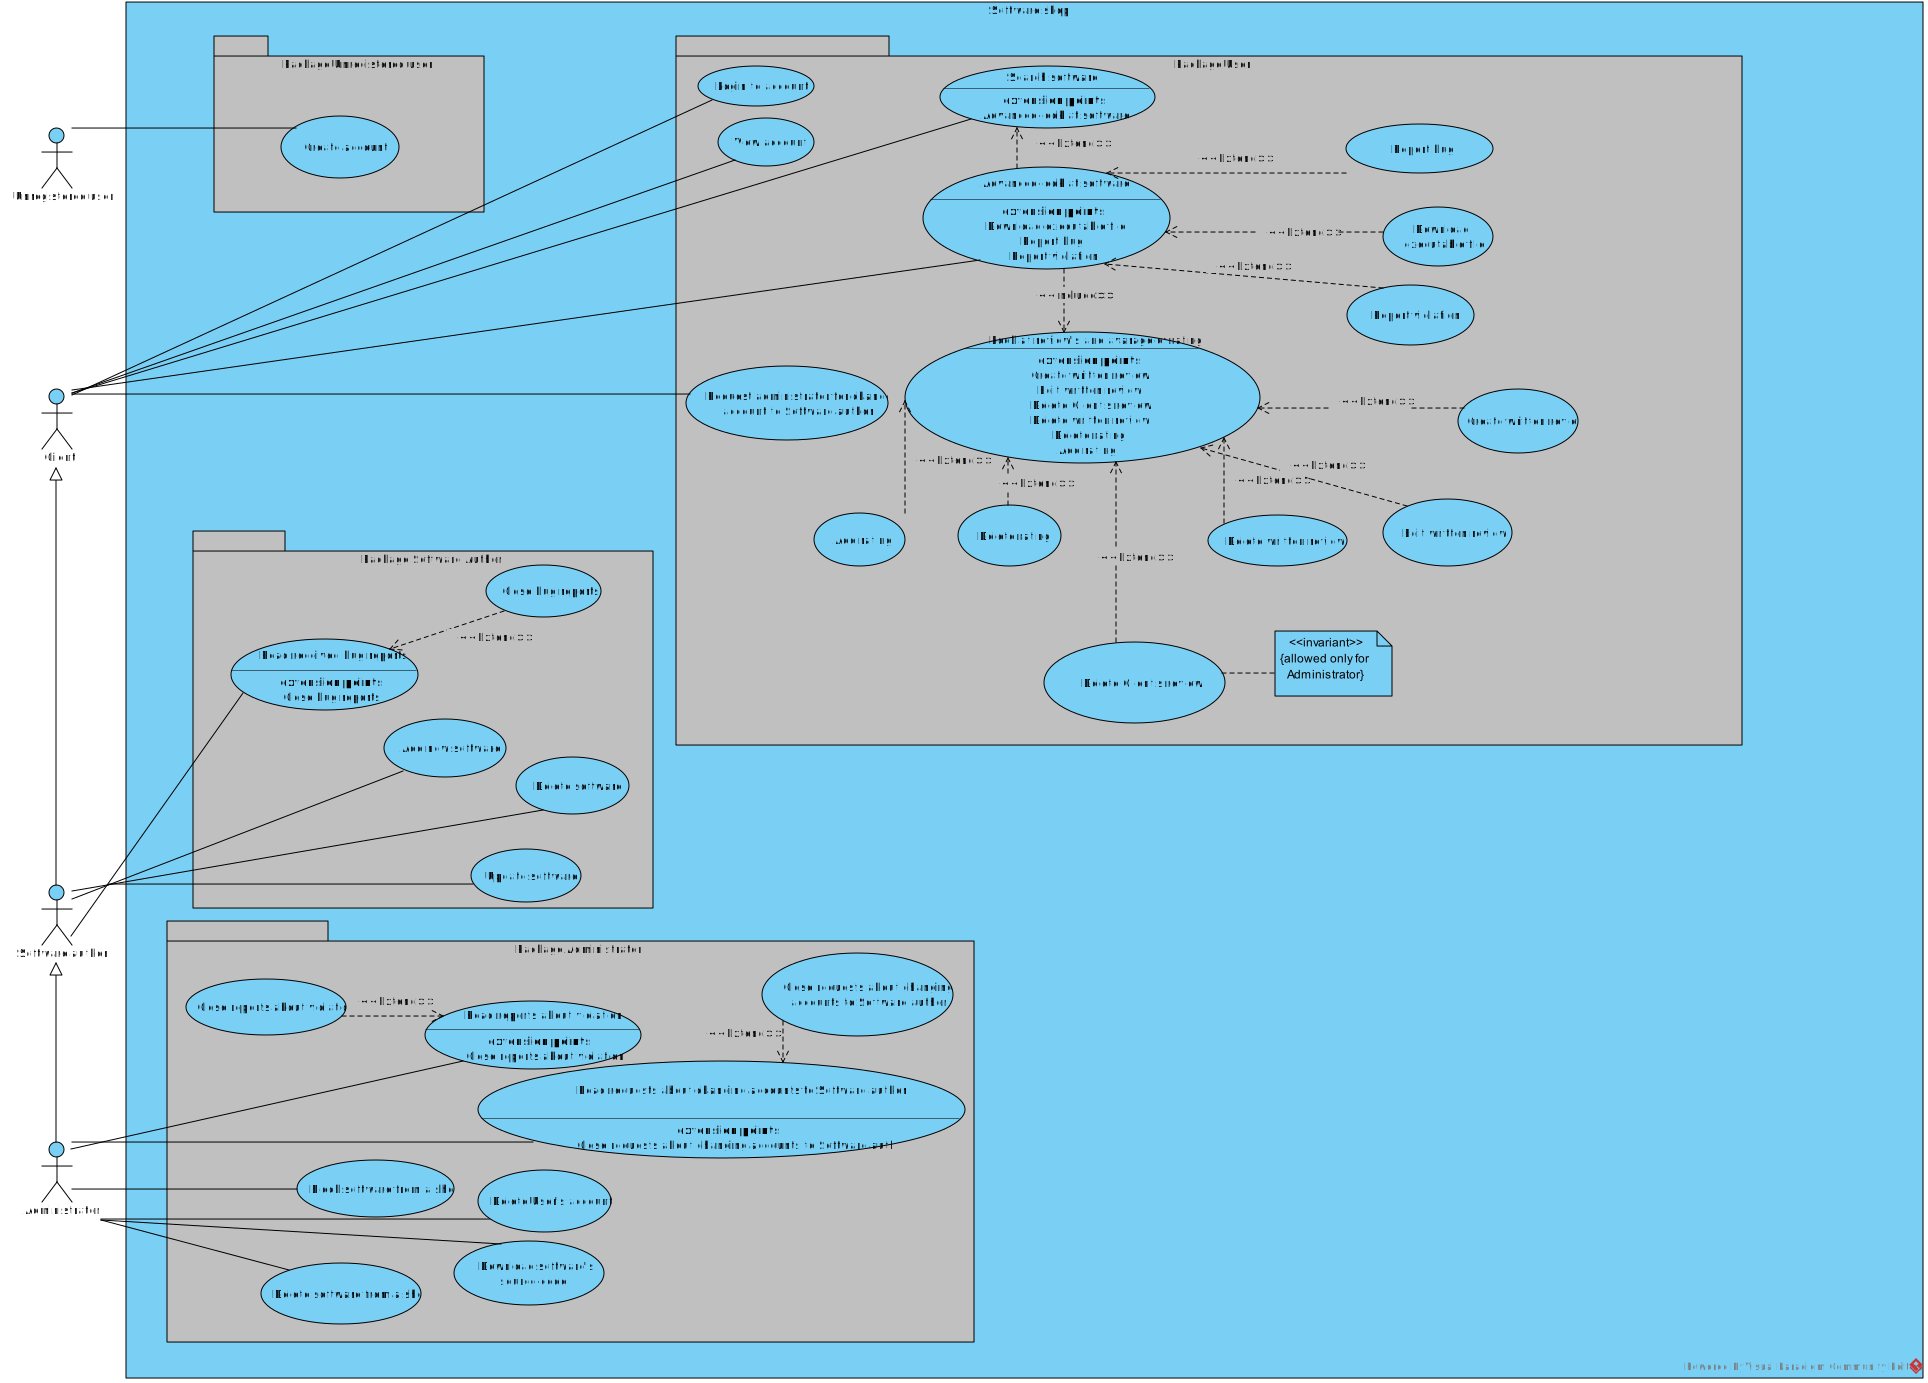
\includegraphics[width=1.35\textwidth]{Diagram przypadków użycia.png}
    }
    \caption{Diagram przypadków użycia}
    \label{fig:diagram_przypadkow}
\end{figure}
\end{document}  